\chapter{Transport optimal}
\label{chap-ot}
\chapteroverview{Comparer deux distributions demande de préciser le coût du déplacement de la masse entre les positions. Le transport optimal traduit cette idée en un problème d'optimisation. À partir d'un petit problème d'affectation, nous introduisons les plans de transport, expliquons quand ils correspondent à des applications, puis utilisons les distances de transport pour comparer des couleurs, des formes et des textes.}

\section{Le problème de Monge}
En 1781, Gaspard Monge formule le problème du déplacement de terre d'un lieu à un autre à moindre coût~\cite{Monge1781}. Son coût est la distance parcourue par chaque unité de masse. D'autres applications suggèrent d'autres coûts, comme le temps de trajet ou le carré de la distance euclidienne.

\subsection{Un problème d'affectation}
Considérons six boulangeries et six cafés à Paris. Chaque boulangerie fournit un lot de croissants, et chaque café demande un lot. Dans le modèle d'affectation, chaque lot va à un seul café, et chaque café reçoit un seul lot. Les deux exigences sont nécessaires : donner simplement une destination à chaque boulangerie permettrait à plusieurs d'entre elles de choisir le même café.

Notons $C_{ij}$ le temps de trajet de la boulangerie $i$ au café $j$. Dans l'exemple de la figure~\ref{fig:image-cafe}, on a $C_{34}=10$. Une affectation admissible est une permutation $\sigma$ de $\{1,\ldots,6\}$. Par exemple,
\begin{equation}\label{eq-bijection-exmp}
 (\sigma(1),\ldots,\sigma(6))=(5,2,6,1,3,4).
\end{equation}
Son coût total est
\begin{equation}\label{eq:cout}
 \text{Coût}(\sigma)=\sum_{i=1}^6 C_{i,\sigma(i)}
 =10+7+15+10+14+9=65.
\end{equation}
On additionne ici les six temps de trajet. Ce modèle ne décrit ni la tournée d'un véhicule unique, ni la durée totale de livraisons effectuées en parallèle.

\begin{figure}[htbp]\centering
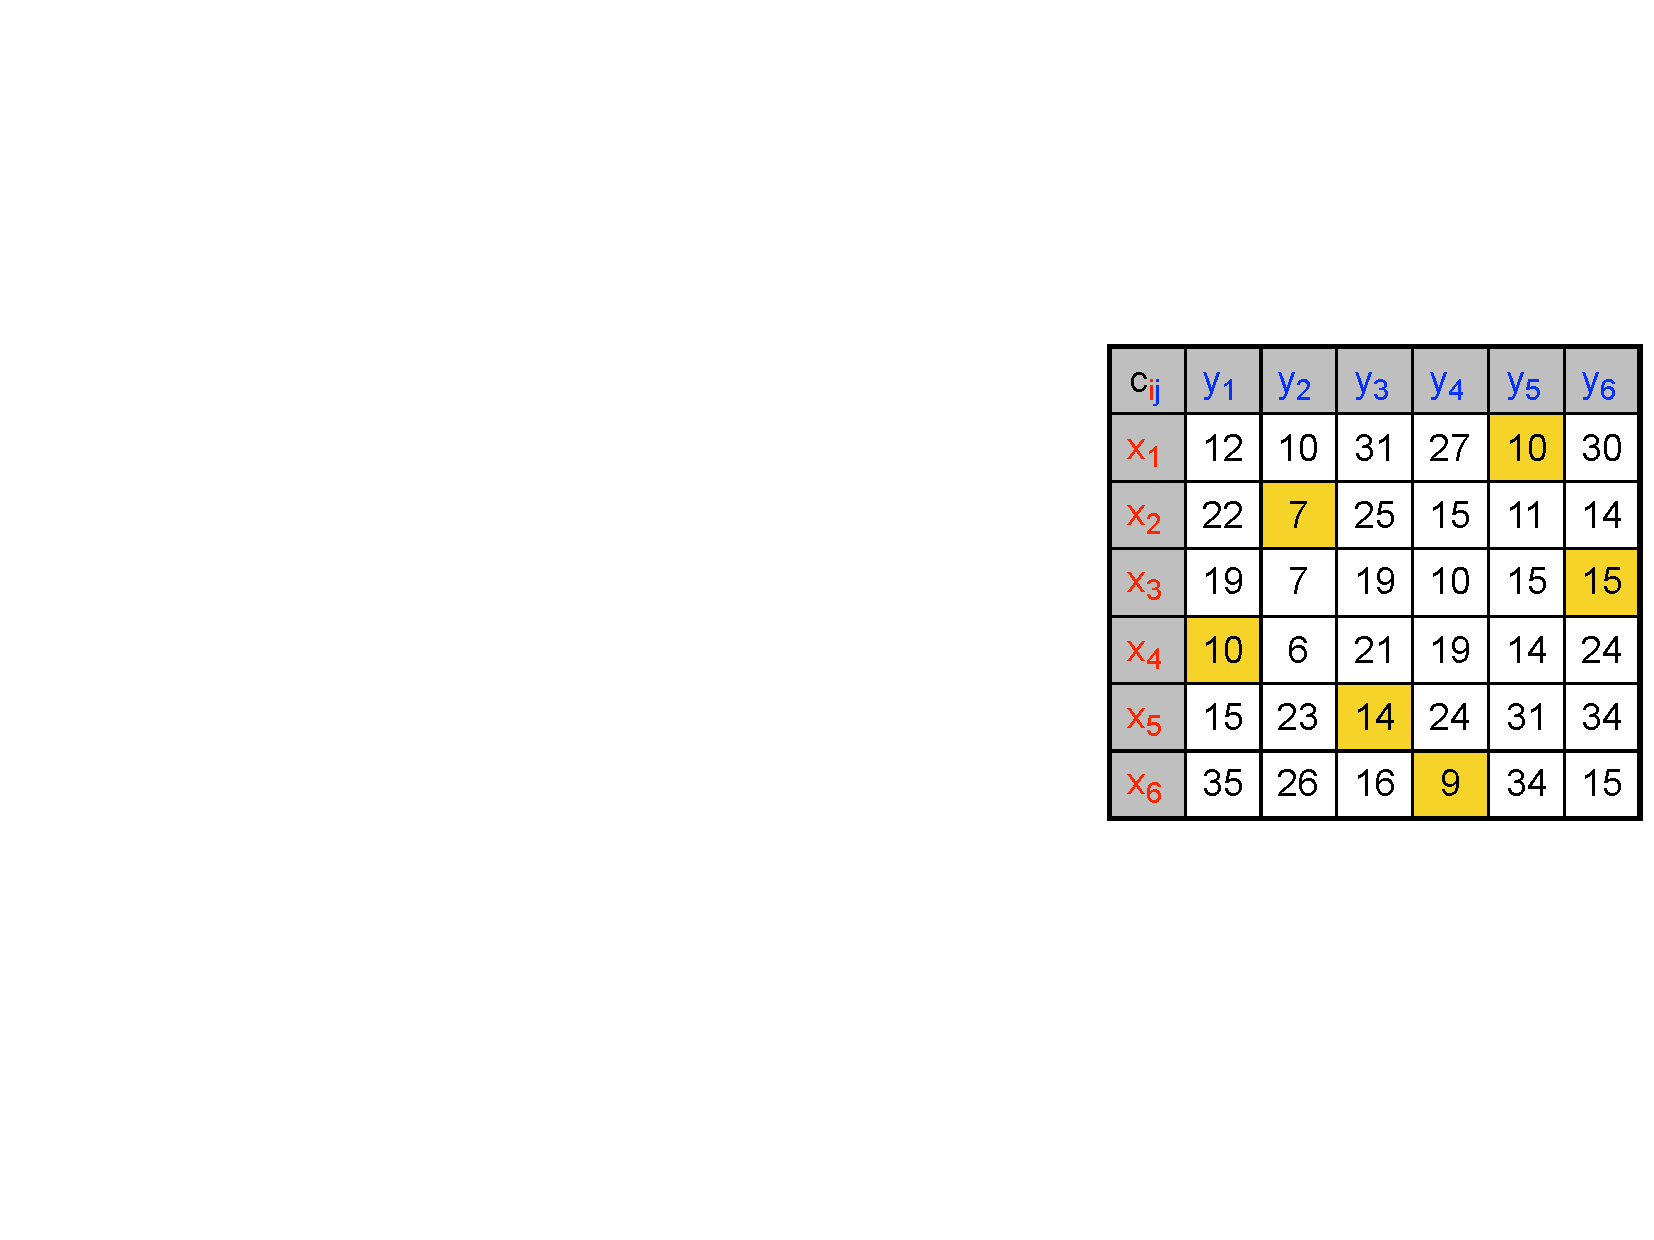
\includegraphics[width=.43\linewidth]{transport-hd/cafe-paris/map-paris-1-couts}\hfill
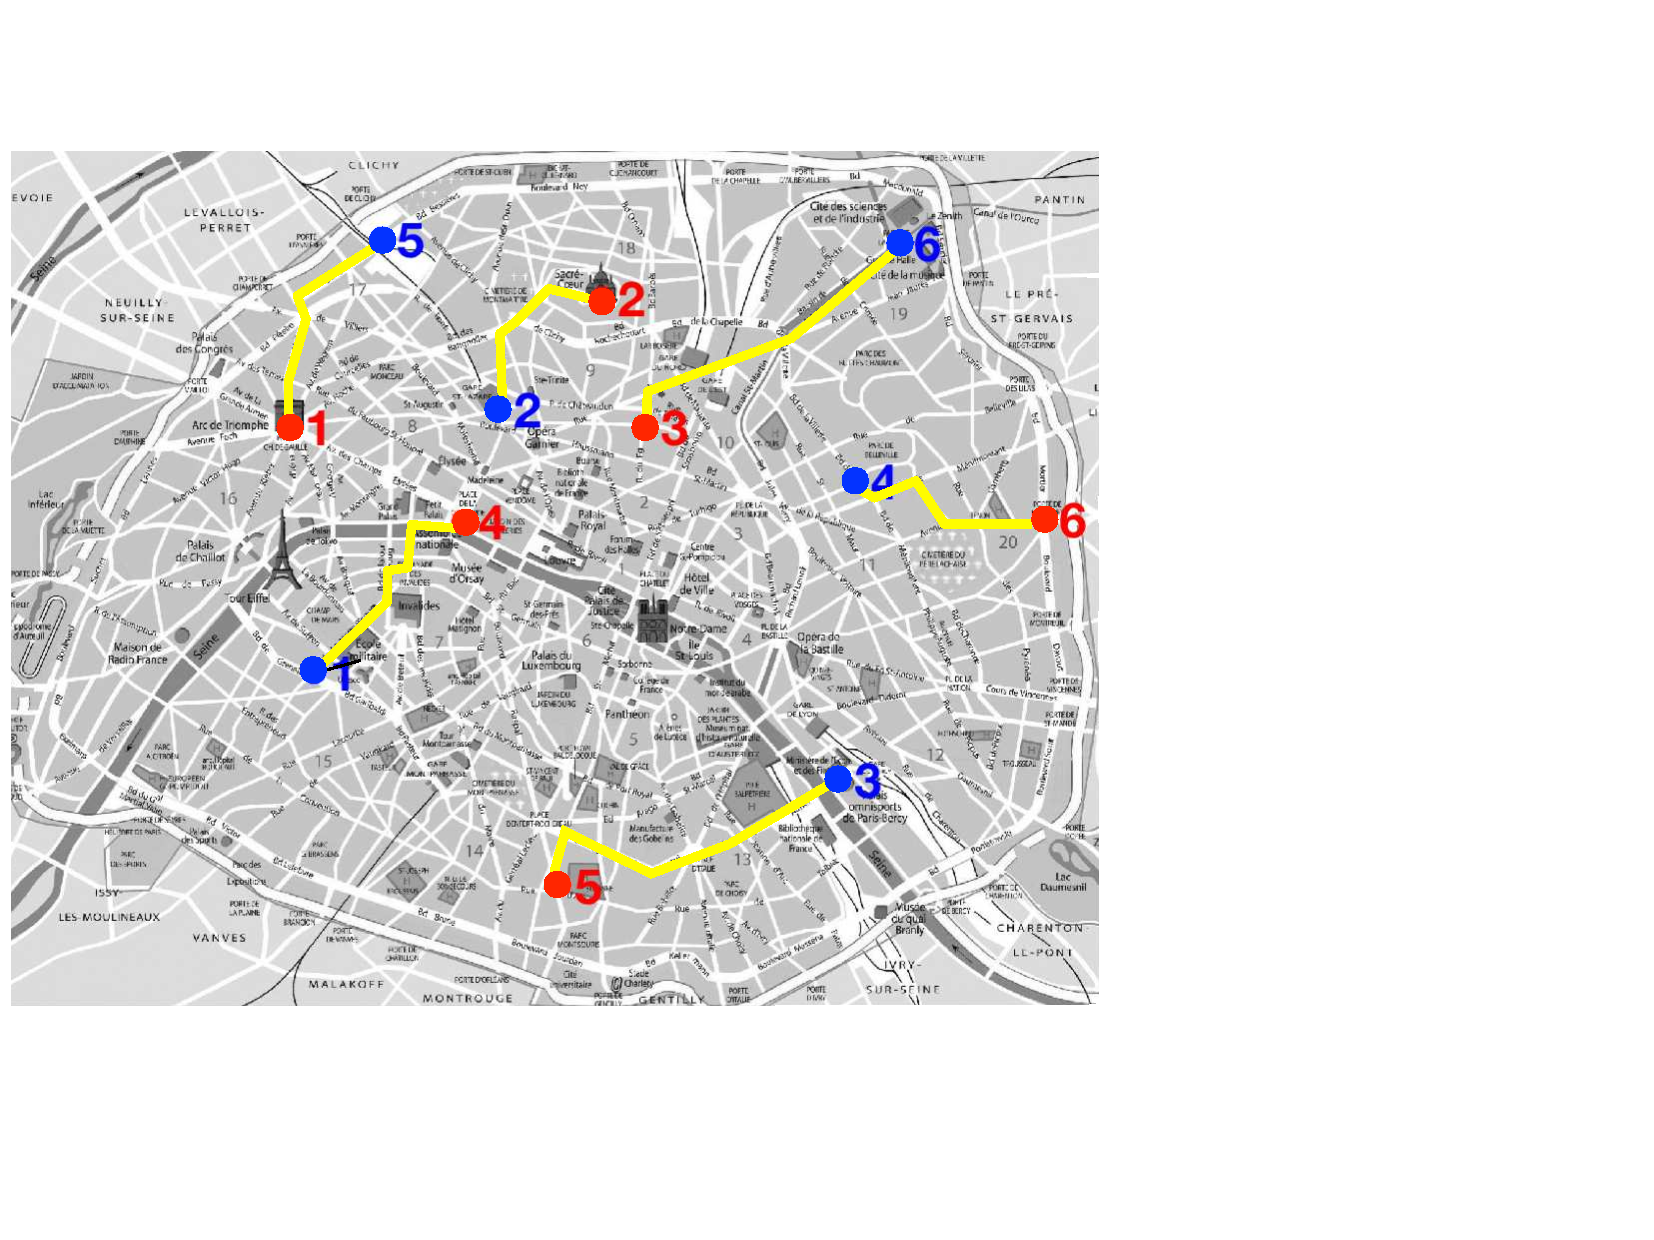
\includegraphics[width=.53\linewidth]{transport-hd/cafe-paris/map-paris-1}
\caption{Matrice de coût et affectation des six boulangeries (rouge) aux six cafés (bleu). Les entrées surlignées donnent un temps de trajet cumulé de 65 minutes.}\label{fig:image-cafe}
\end{figure}

Pour $n$ lots identiques de chaque côté, le problème discret de Monge s'écrit
\begin{equation}\label{eq:monge}
 \min_{\sigma\in\Sigma_n}\sum_{i=1}^n C_{i,\sigma(i)},
\end{equation}
où $\Sigma_n$ est l'ensemble des permutations. Dans notre exemple, la valeur optimale est 64, atteinte par $(5,6,2,1,3,4)$. L'examen exhaustif des $6!=720$ possibilités permet de le vérifier. Il y a $n!$ affectations en général, et $70!\approx1{,}198\times10^{100}$ : l'énumération devient donc vite impraticable.

\begin{figure}[htbp]\centering
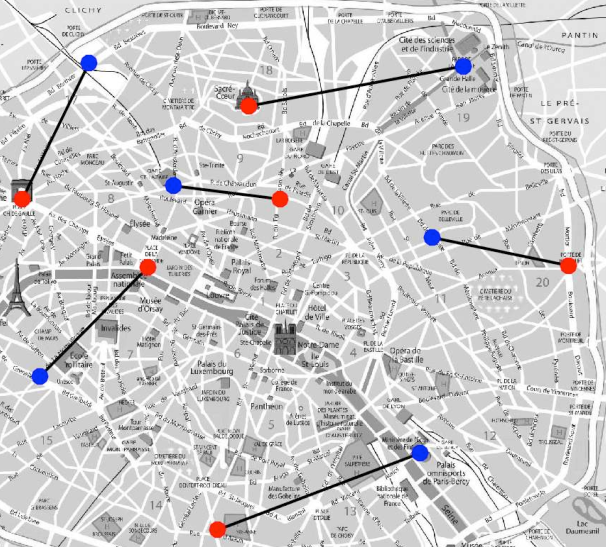
\includegraphics[width=.235\linewidth]{transport-hd/cafe-paris/ordre-croissant-64}\hfill
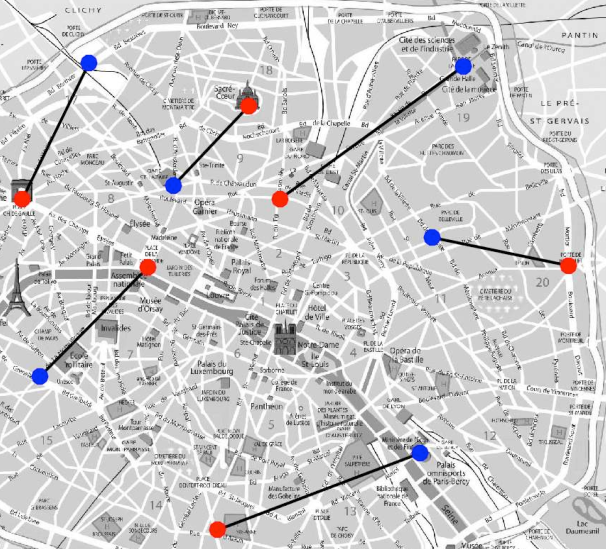
\includegraphics[width=.235\linewidth]{transport-hd/cafe-paris/ordre-croissant-65}\hfill
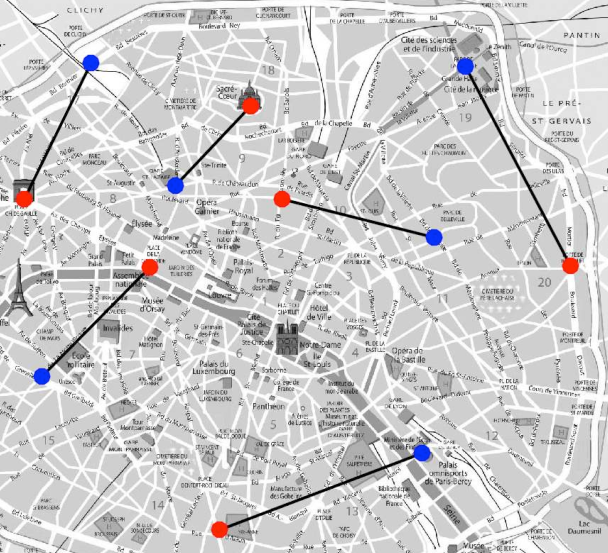
\includegraphics[width=.235\linewidth]{transport-hd/cafe-paris/ordre-croissant-66}\hfill
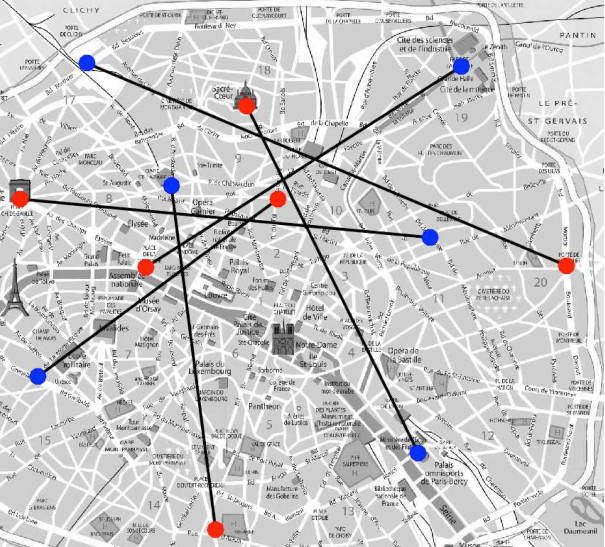
\includegraphics[width=.235\linewidth]{transport-hd/cafe-paris/ordre-croissant-152}
\caption{Quatre affectations de coûts 64, 65, 66 et 152, de gauche à droite.}\label{fig:order-increasing}
\end{figure}

\subsection{Trier en dimension un}
Supposons que les positions sources $x_1\le\cdots\le x_n$ et cibles $y_1\le\cdots\le y_n$ soient sur une droite, avec le coût $C_{ij}=|x_i-y_j|$. Apparier les points dans l'ordre croissant est optimal. L'inégalité essentielle est
\[
 |x-y|+|x'-y'|\le |x-y'|+|x'-y|
 \quad\text{si }x\le x'\text{ et }y\le y'.
\]
On la vérifie en ordonnant les quatre points sur la droite. Lorsqu'une permutation contient une inversion, échanger les deux destinations n'augmente pas le coût. Éliminer successivement les inversions donne l'appariement trié. Une égalité est possible : cette affectation optimale n'est donc pas nécessairement unique.

\begin{figure}[htbp]\centering
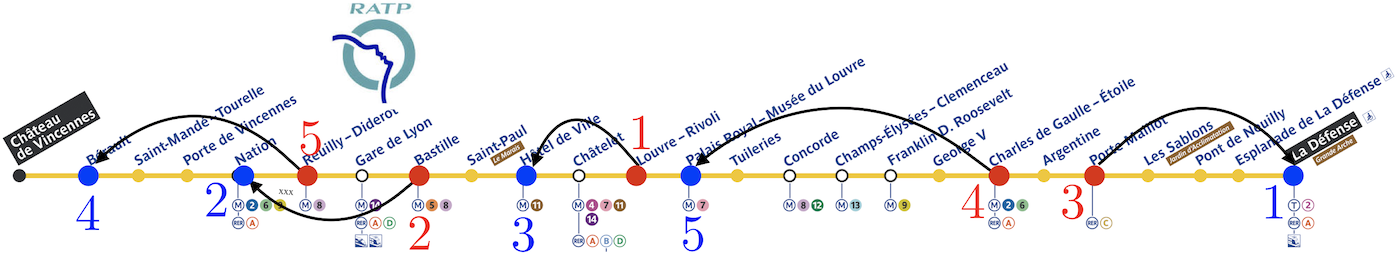
\includegraphics[width=.97\linewidth]{transport-hd/metro/plan-metro}
\caption{Appariement trié le long d’une ligne de métro, considérée comme un axe unidimensionnel. Pour les indices affichés, $\sigma:(1,2,3,4,5)\mapsto(3,2,1,5,4)$.}\label{fig:metro}
\end{figure}

Le coût du calcul est ainsi celui du tri des deux listes. Le tri par insertion effectue au plus $n(n-1)/2$ comparaisons par liste, soit 2\,415 pour $n=70$. Le tri fusion ramène ce coût à l'ordre de $n\log n$. Il s'agit du nombre de comparaisons pour le tri, et non d'une estimation de toutes les opérations d'une application de transport.

En dimension deux, aucun ordre unique ne résout le problème général. Pour le coût euclidien, deux segments d'un appariement optimal ne peuvent toutefois pas se croiser transversalement en leurs intérieurs. Si les segments $[x,y]$ et $[x',y']$ se rencontrent en $z$, l'inégalité triangulaire donne
\[
 |x-y'|+|x'-y|\le |x-z|+|z-y'|+|x'-z|+|z-y|
 =|x-y|+|x'-y'|.
\]
Pour un croisement transverse, l'inégalité est stricte : échanger les destinations diminue le coût. Des recouvrements colinéaires ou des extrémités communes sont des cas dégénérés qui ne donnent pas nécessairement d'amélioration stricte. Cette observation ne suffit pas à calculer un optimum : de nombreux appariements sans croisement peuvent avoir des coûts différents.

\begin{figure}[htbp]\centering
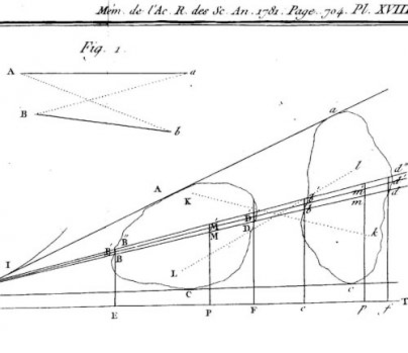
\includegraphics[width=.30\linewidth]{transport-hd/monge-2d/article-monge}\hfill
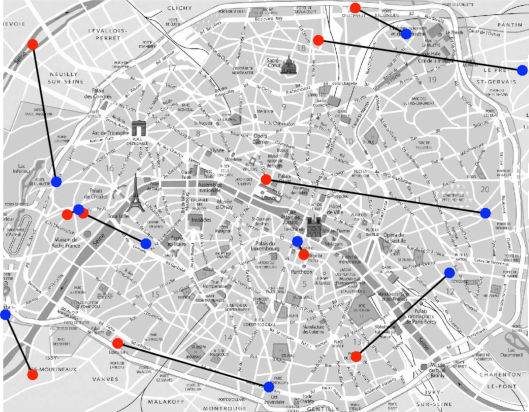
\includegraphics[width=.30\linewidth]{transport-hd/monge-2d/example-10}\hfill
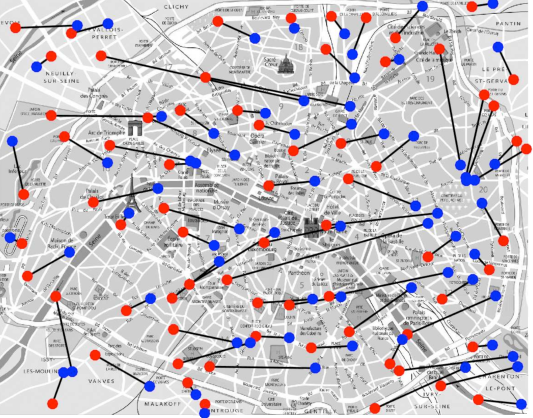
\includegraphics[width=.30\linewidth]{transport-hd/monge-2d/example-70}
\caption{Une illustration de l’article original de Monge~\cite{Monge1781} et deux appariements euclidiens optimaux dans le plan.}\label{fig:ot2d}
\end{figure}

\section{La relaxation de Kantorovitch}
\label{sec-kanto}
La formulation de Kantorovitch autorise le partage de la masse entre plusieurs destinations~\cite{Kantorovich42}. Elle remplace les choix discrets par des quantités positives ou nulles soumises à des contraintes linéaires de conservation, faisant du transport optimal un problème de programmation linéaire.

\subsection{Des permutations aux matrices}
On représente une permutation par $P_{ij}=1$ si $j=\sigma(i)$ et $P_{ij}=0$ sinon. Par exemple, les permutations $(1,2,3)$, $(3,2,1)$ et $(2,1,3)$ correspondent à
\[
 \begin{pmatrix}1&0&0\\0&1&0\\0&0&1\end{pmatrix},\qquad
 \begin{pmatrix}0&0&1\\0&1&0\\1&0&0\end{pmatrix},\qquad
 \begin{pmatrix}0&1&0\\1&0&0\\0&0&1\end{pmatrix}.
\]
Chaque ligne et chaque colonne a pour somme un. Si $\mathcal P_n$ désigne l'ensemble de ces matrices de permutation, le problème~\eqref{eq:monge} équivaut à
\begin{equation}\label{eq:mongematrix}
 \min_{P\in\mathcal P_n}\langle C,P\rangle,
 \qquad \langle C,P\rangle=\sum_{i,j}C_{ij}P_{ij}.
\end{equation}
Relâcher la contrainte binaire donne les matrices bistochastiques
\begin{equation}\label{eq:bistoch}
 \mathcal B_n=\left\{P\in\RR_+^{n\times n}:\sum_jP_{ij}=1,\ \sum_iP_{ij}=1\right\}.
\end{equation}
La positivité et les sommes des lignes impliquent déjà $P_{ij}\le1$. Le problème relaxé est
\begin{equation}\label{eq:kantoassign}
 \min_{P\in\mathcal B_n}\langle C,P\rangle.
\end{equation}
L'ensemble $\mathcal B_n$ est compact et convexe : pour $P,Q\in\mathcal B_n$ et $0\le t\le1$, la matrice $(1-t)P+tQ$ reste admissible. Un minimiseur existe car l'objectif est continu.

Le développement de la programmation linéaire, notamment de la méthode du simplexe de Dantzig~\cite{Dantzig51}, a rendu ces problèmes accessibles au calcul. Des algorithmes d'affectation spécialisés, comme certaines implémentations de la méthode hongroise, résolvent le problème dense $n\times n$ en $O(n^3)$ opérations. Cette borne ne doit pas être attribuée à la méthode générale du simplexe, dont le temps de calcul dans le pire cas n'est pas polynomial.

\subsection{Pourquoi la relaxation est exacte pour des masses égales}
Le théorème de Birkhoff--von Neumann affirme que toute matrice bistochastique est une combinaison convexe de matrices de permutation~\cite{birkhoff,von1953certain} :
\[
 P=\sum_{k=1}^K\lambda_k P^{(k)},
 \qquad \lambda_k\ge0,\quad\sum_k\lambda_k=1.
\]
Ainsi, $\langle C,P\rangle=\sum_k\lambda_k\langle C,P^{(k)}\rangle$ ne peut pas être inférieur au plus petit coût d'une permutation. Comme toute matrice de permutation est admissible pour la relaxation, on obtient
\begin{equation}\label{eq:monge-vs-kanto}
 \min_{P\in\mathcal B_n}\langle C,P\rangle
 =\min_{P\in\mathcal P_n}\langle C,P\rangle.
\end{equation}
Au moins un plan optimal est donc une permutation. Cela ne signifie pas que tout plan optimal soit une permutation : la moyenne de deux permutations optimales distinctes est également optimale. Si tous les coûts sont nuls, toute matrice bistochastique est optimale.

Pour certifier une valeur optimale, on peut chercher des nombres $u_i,v_j$ tels que $u_i+v_j\le C_{ij}$. Toute matrice $P\in\mathcal B_n$ vérifie alors
\[
 \langle C,P\rangle\ge\sum_{i,j}(u_i+v_j)P_{ij}=\sum_i u_i+\sum_jv_j.
\]
Dans l'exemple parisien, $u=(2,3,3,0,5,2)$ et $v=(10,4,9,7,8,11)$ vérifient les 36 inégalités et la somme de leurs composantes vaut 64. Avec une affectation de coût 64, ils prouvent donc l'optimalité sans énumérer toutes les permutations.

\subsection{Des nombres de points et des masses différents}
Supposons maintenant que $n$ boulangeries fournissent des quantités $a_i\ge0$ et que $m$ cafés demandent des quantités $b_j\ge0$, avec la même masse totale
\[
 \sum_{i=1}^n a_i=\sum_{j=1}^m b_j=s.
\]
Un plan de transport appartient à
\[
 \mathcal B(a,b)=\left\{P\in\RR_+^{n\times m}:\sum_jP_{ij}=a_i,\ \sum_iP_{ij}=b_j\right\}.
\]
Pour $s>0$, le plan $P_{ij}=a_i b_j/s$ prouve que cet ensemble est non vide. Pour $s=0$, le seul plan est nul. Le problème de transport s'écrit
\begin{equation}\label{eq-kanto-gen}
 \min_{P\in\mathcal B(a,b)}\sum_{i=1}^n\sum_{j=1}^m C_{ij}P_{ij}.
\end{equation}
Pour des coûts finis, la compacité assure encore l'existence d'un minimiseur. L'entrée $P_{ij}$ est la quantité expédiée de $i$ vers $j$, et $C_{ij}$ son coût par unité de masse.

\begin{figure}[htbp]\centering
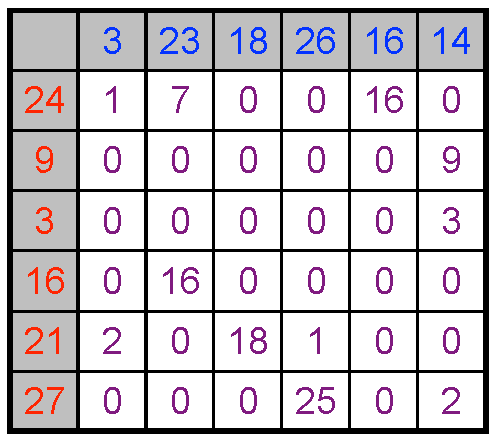
\includegraphics[width=.235\linewidth]{transport-hd/kantorovitch/coupling-array}\hfill
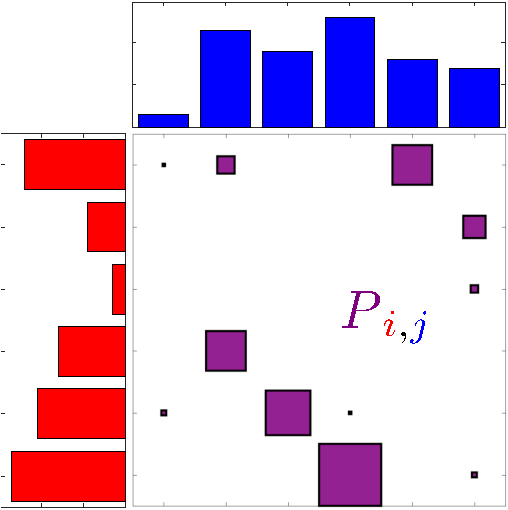
\includegraphics[width=.235\linewidth]{transport-hd/kantorovitch/coupling-squares}\hfill
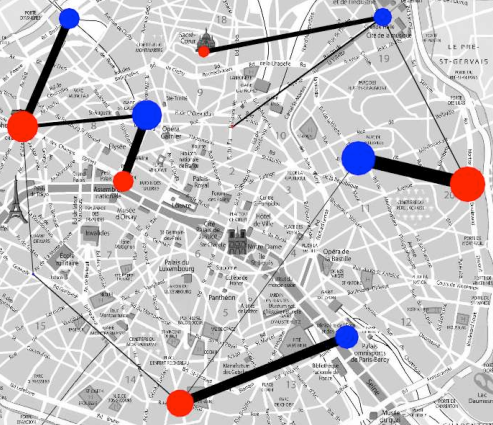
\includegraphics[width=.235\linewidth]{transport-hd/kantorovitch/coupling-map}\hfill
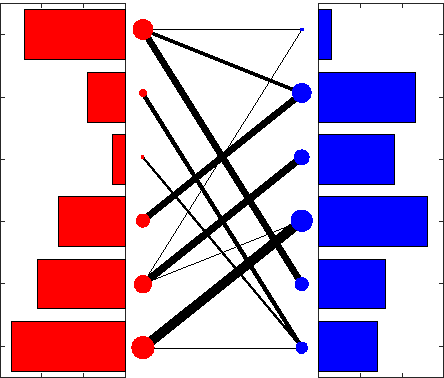
\includegraphics[width=.235\linewidth]{transport-hd/kantorovitch/coupling-bipartite}
\caption{Quatre représentations du même couplage : ses entrées matricielles, leurs amplitudes représentées par des carrés, des segments pondérés dans l’espace et un graphe biparti. Les sommes des lignes et des colonnes donnent les masses prescrites $a$ et $b$.}\label{fig:coupling-visu}
\end{figure}

Le partage de la masse peut devenir nécessaire. Une boulangerie de masse 2 et deux cafés demandant chacun une masse 1 admettent pour seul plan $P=(1\;1)$. Une application qui envoie toute la masse source vers une seule cible ne peut pas réaliser ces marginales. Un plan de transport est donc plus général qu'une application de transport. Pour des masses égales $a_i=b_j=1$, on retrouve $\mathcal B_n$ ; pour des masses de probabilité $a_i=b_j=1/n$, les plans correspondants sont les $P/n$.

\section{Mesures et distances de transport}
Les mêmes idées s'appliquent aux mesures de probabilité, notamment aux distributions discrètes $\mu=\sum_i a_i\delta_{x_i}$ et $\nu=\sum_jb_j\delta_{y_j}$. Un couplage $\pi\in\Pi(\mu,\nu)$ est une mesure de probabilité sur les couples $(x,y)$ dont les marginales sont $\mu$ et $\nu$. Une application mesurable $T$ induit un couplage $(\mathrm{Id},T)_\#\mu$ lorsque $T_\#\mu=\nu$ ; cette notation signifie qu'appliquer $T$ à une variable aléatoire de loi $\mu$ donne une variable de loi $\nu$.

Pour des mesures de probabilité sur $\RR^d$ à moments d'ordre deux finis, la distance de transport quadratique est
\begin{equation}\label{eq-wasserstein}
 W_2(\mu,\nu)^2=\min_{\pi\in\Pi(\mu,\nu)}\int |x-y|^2\,\d\pi(x,y).
\end{equation}
Dans le cas discret, on retrouve~\eqref{eq-kanto-gen} avec $C_{ij}=|x_i-y_j|^2$. La distance dépend des masses et des positions : des vecteurs de poids égaux placés à des endroits différents ne décrivent pas nécessairement la même mesure. La racine carrée $W_2$ est une distance, et $W_2(\mu,\nu)=0$ exactement lorsque $\mu=\nu$. Son carré ne vérifie généralement pas l'inégalité triangulaire : pour des masses de Dirac en 0, 1 et 2, les distances au carré correspondantes valent 1, 1 et 4.

Le théorème de Brenier précise une condition sous laquelle le couplage optimal est une application~\cite{Brenier91}. Si la source $\mu$ est absolument continue par rapport à la mesure de Lebesgue et si les deux mesures ont des moments d'ordre deux finis, le problème quadratique admet un unique couplage optimal. Il est induit par une application $T=\nabla\varphi$, où $\varphi$ est convexe, et $T$ est unique $\mu$-presque partout. L'absolue continuité et le choix du coût sont essentiels ; on ne peut pas affirmer cette conclusion pour des mesures et des coûts arbitraires.

\section{Applications}
\subsection{Transférer une palette de couleurs}
Pour deux images ayant le même nombre $n$ de pixels, notons $x_i,y_j\in\RR^3$ leurs couleurs RVB. Une affectation minimisant $\sum_i|x_i-y_{\sigma(i)}|^2$ donne une image dont la couleur à la position source $i$ est $y_{\sigma(i)}$. Chaque couleur cible est utilisée une fois : la sortie possède donc exactement la distribution empirique des couleurs de la cible. L'optimisation limite les changements de couleur, mais ne comporte aucun terme de régularité spatiale ; la préservation des contours et des textures n'est donc pas garantie.

\begin{figure}[htbp]\centering
\begin{tabular}{@{}ccc@{}}
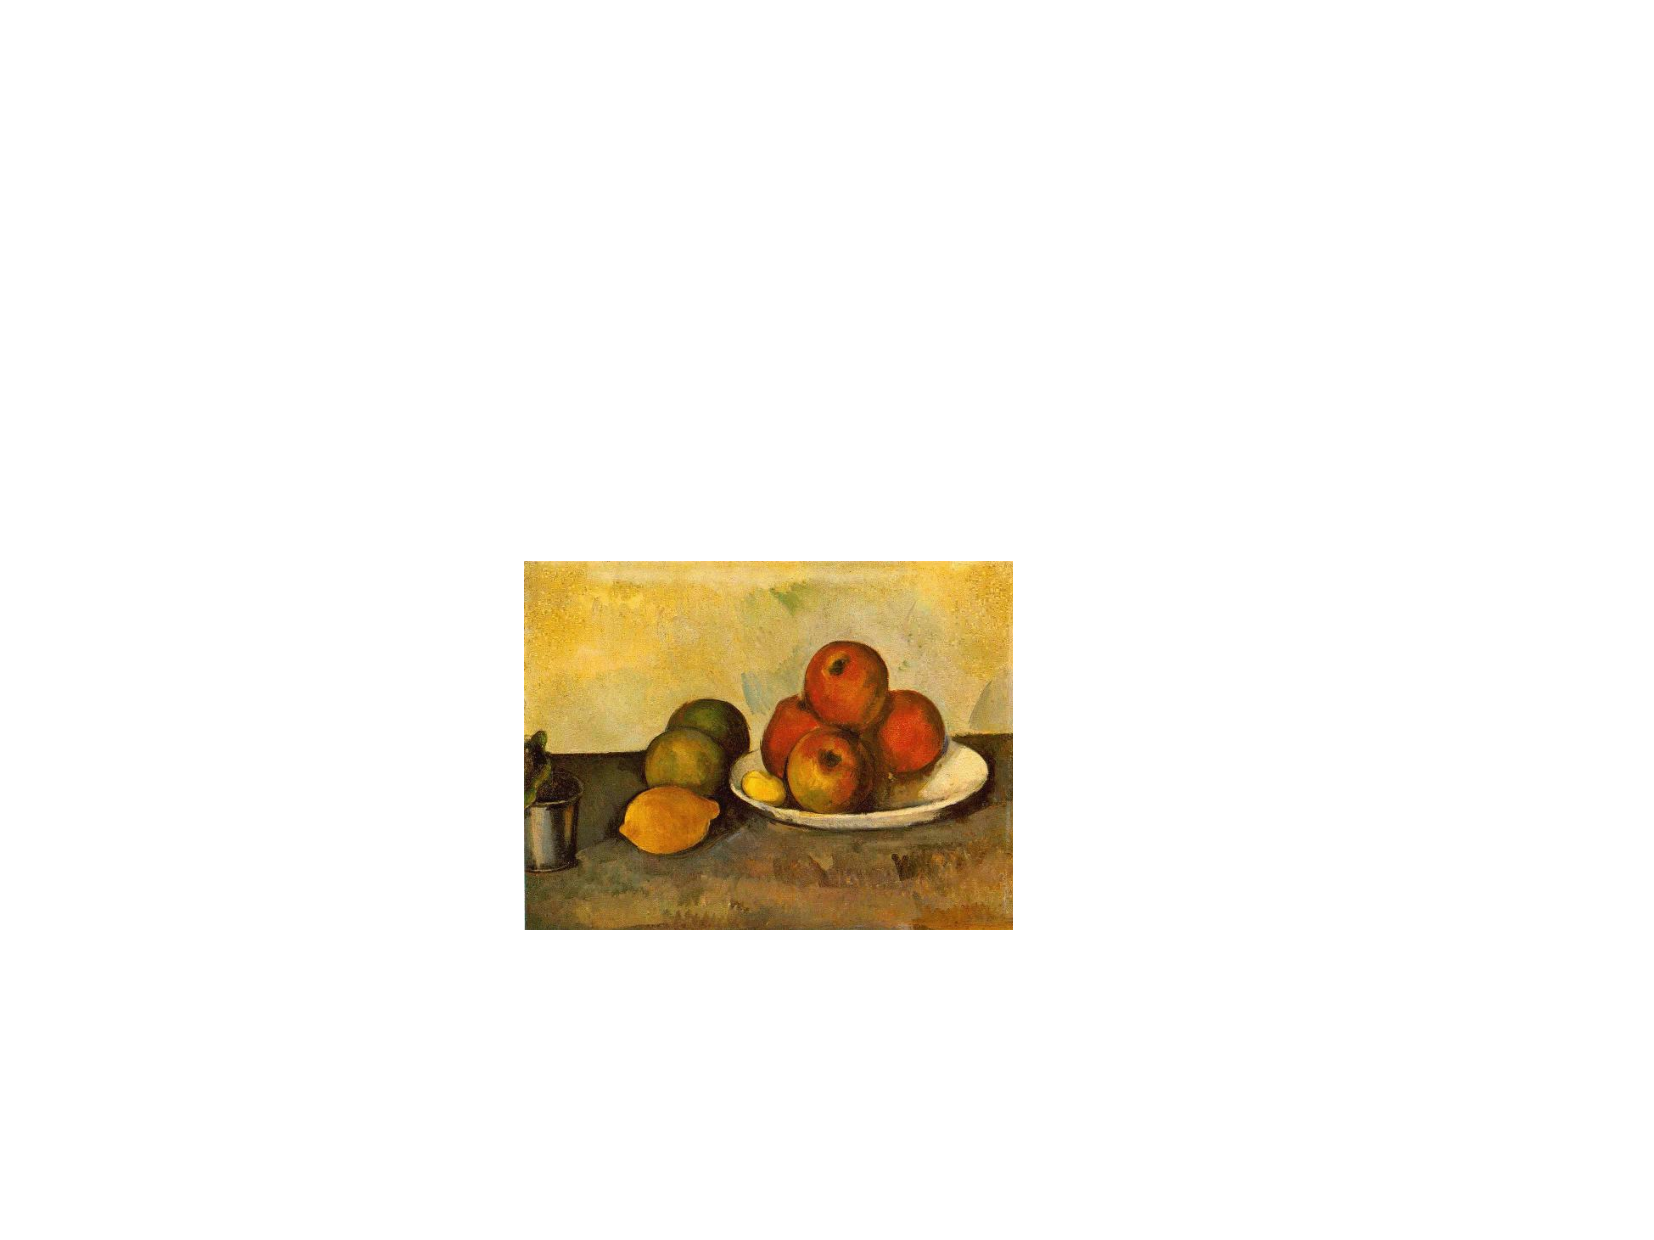
\includegraphics[width=.29\linewidth]{transport-hd/applis/painting-2} &
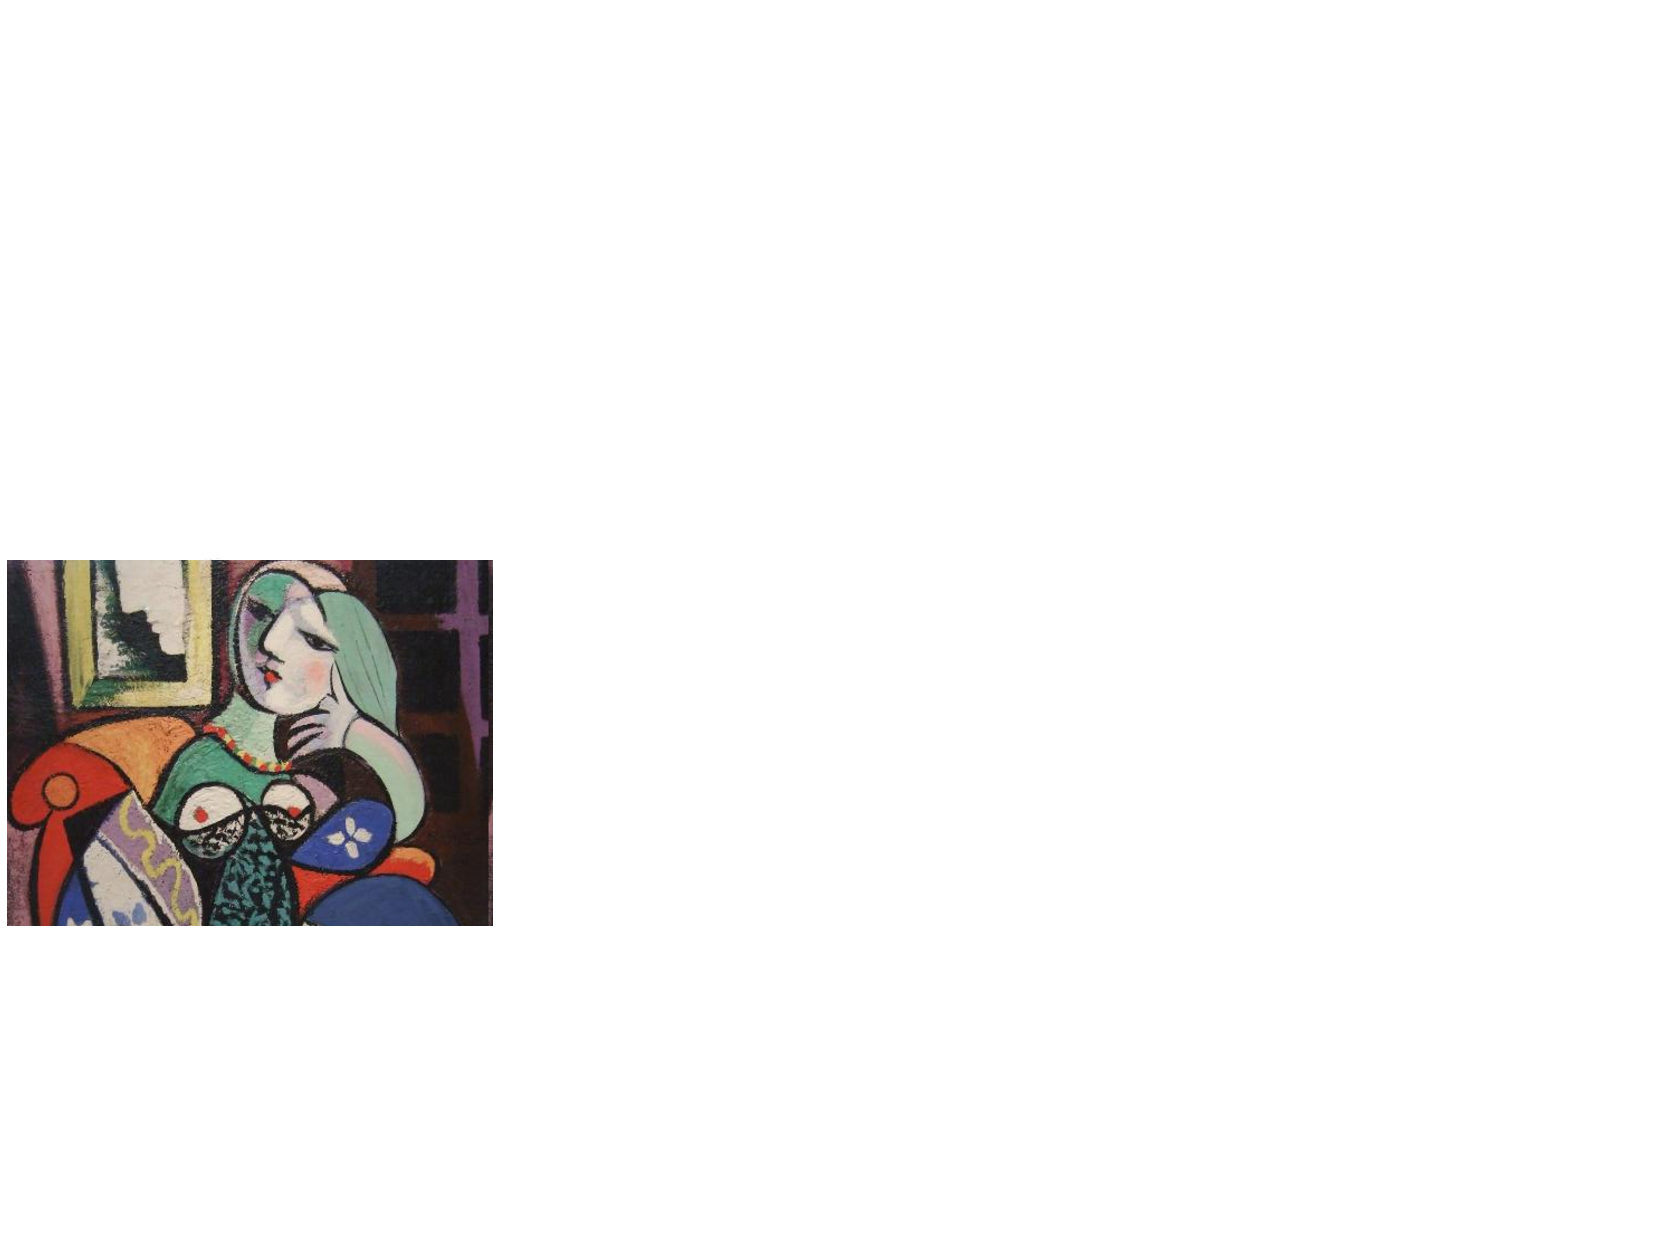
\includegraphics[width=.29\linewidth]{transport-hd/applis/painting-1} &
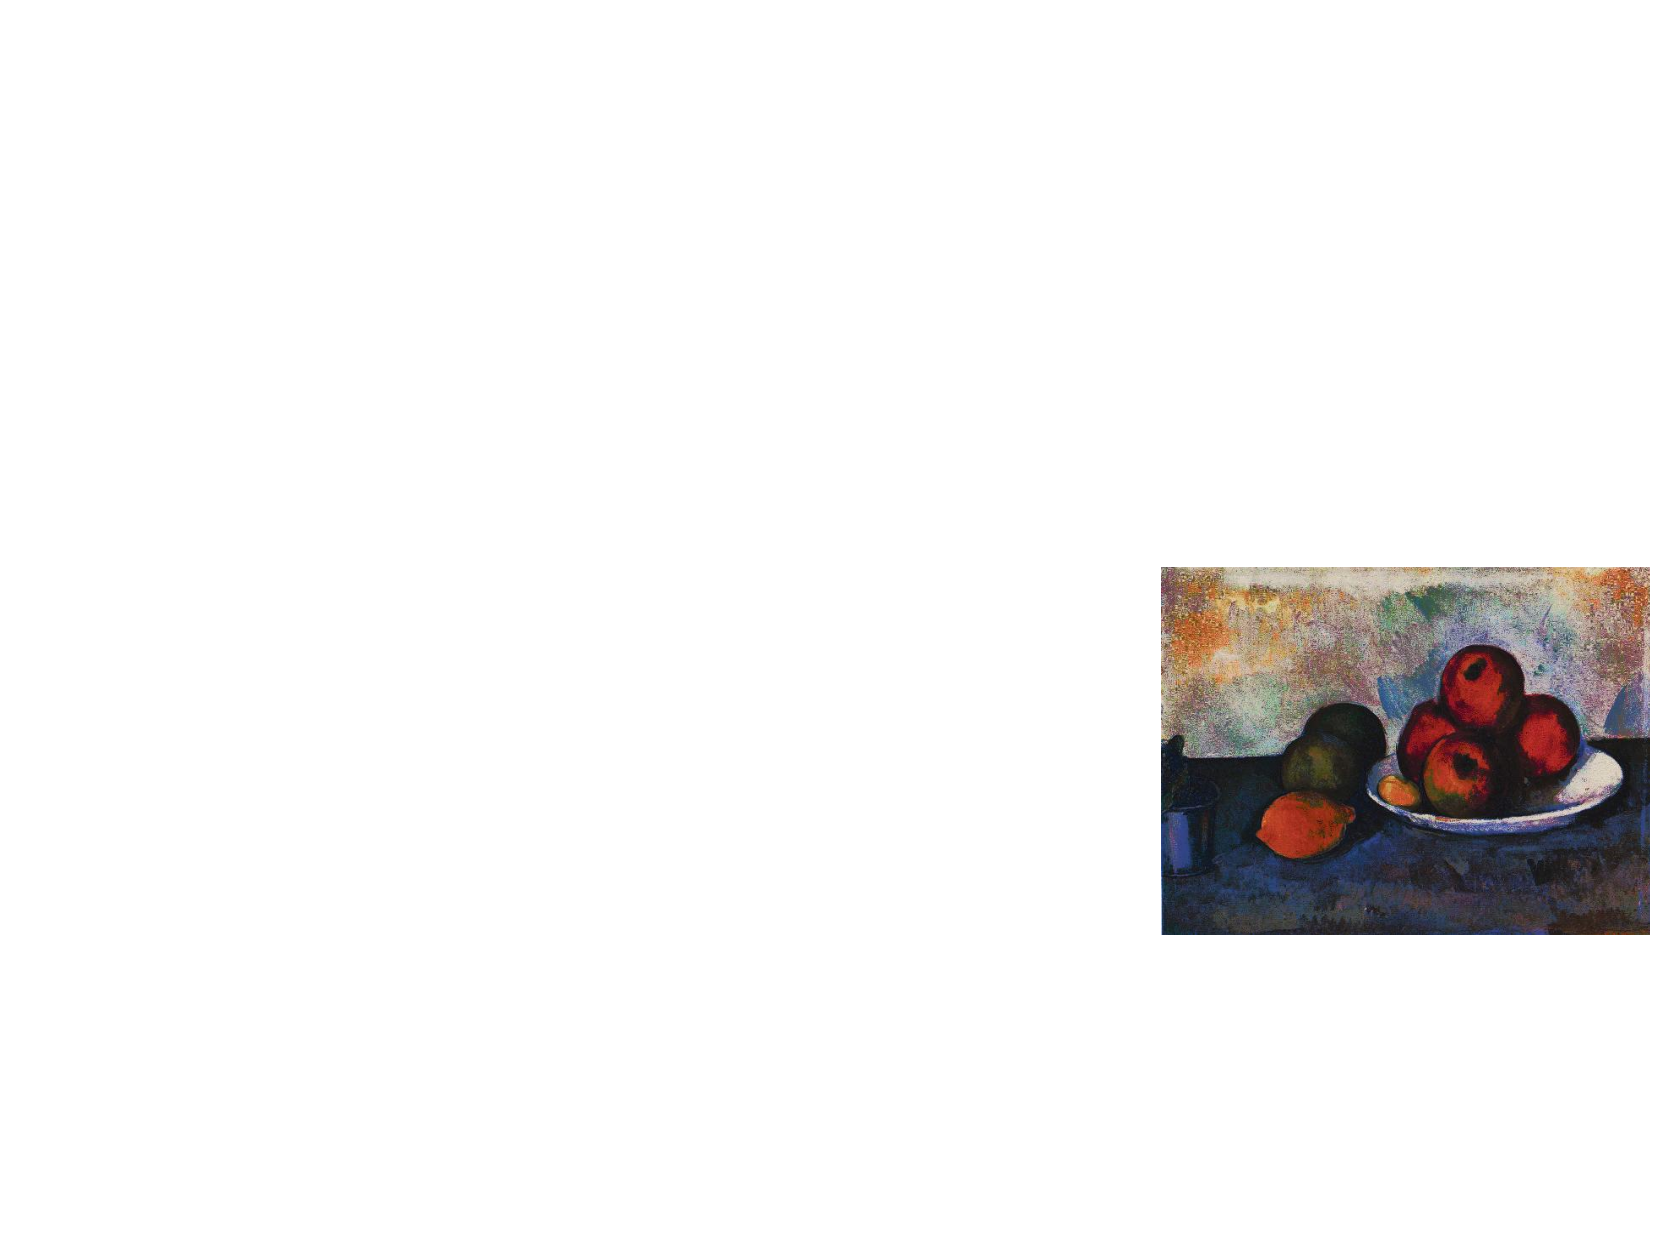
\includegraphics[width=.29\linewidth]{transport-hd/applis/painting-2-equalized}\\[3pt]
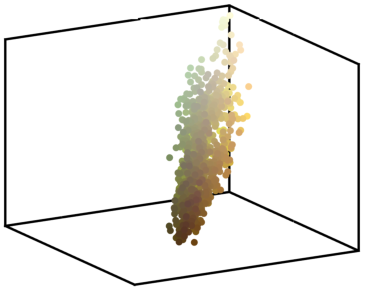
\includegraphics[width=.29\linewidth]{transport-hd/applis/painting-2-histo} &
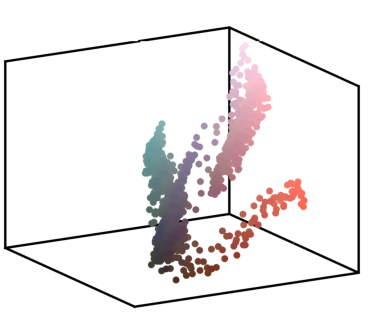
\includegraphics[width=.29\linewidth]{transport-hd/applis/painting-1-histo} &
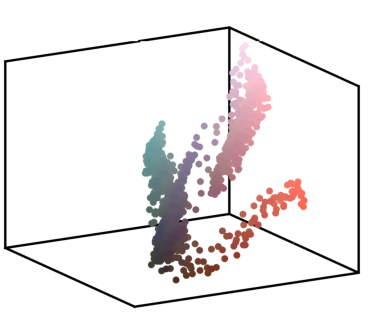
\includegraphics[width=.29\linewidth]{transport-hd/applis/painting-1-histo}
\end{tabular}
\caption{Transfert de palette. Colonnes : source, cible et source recolorée. En haut, les couleurs sur la grille de l’image ; en bas, les nuages de points correspondants dans l’espace RVB. Une permutation des couleurs cibles donne le même nuage dans les deux dernières colonnes.}\label{fig:image-eq}
\end{figure}

Cette distinction sépare le transport de couleurs du déplacement des pixels dans le plan de l'image. Ici, les positions transportées sont des points de l'espace des couleurs ; la grille d'affichage reste fixe. Pour des images de tailles différentes ou des groupes de couleurs pondérés, on utilise un couplage et une règle précisant sa conversion en couleurs de sortie. Une moyenne barycentrique des couleurs couplées ne préserve pas nécessairement l'histogramme cible exact.

\subsection{Barycentres de formes}
La moyenne euclidienne pondérée de trois points minimise $\alpha|x-r|^2+\beta|y-r|^2+\gamma|z-r|^2$, où $\alpha,\beta,\gamma\ge0$ et $\alpha+\beta+\gamma=1$. Elle vaut $r=\alpha x+\beta y+\gamma z$. Remplacer les distances euclidiennes au carré par des distances de transport au carré définit un barycentre de Wasserstein~\cite{agueh2011barycenters} :
\begin{equation}\label{eq-bary}
 \min_{\rho\in\mathcal P_2(\RR^d)}
 \alpha W_2(\mu,\rho)^2+\beta W_2(\nu,\rho)^2+\gamma W_2(\eta,\rho)^2.
\end{equation}
On note $\mathcal P_2$ l'ensemble des mesures de probabilité à moment d'ordre deux fini. Dans un calcul sur une grille, on restreint plutôt $\rho$ à des poids de probabilité sur cette grille. Une forme se représente par une densité uniforme à l'intérieur, normalisée pour avoir une masse totale égale à un. Faire varier les trois poids produit une famille de distributions interpolées (figure~\ref{fig:barycenters}). Ces distributions ne sont pas nécessairement uniformes à l'intérieur d'une forme au contour net, et leur unicité demande des hypothèses supplémentaires.

\begin{figure}[htbp]\centering
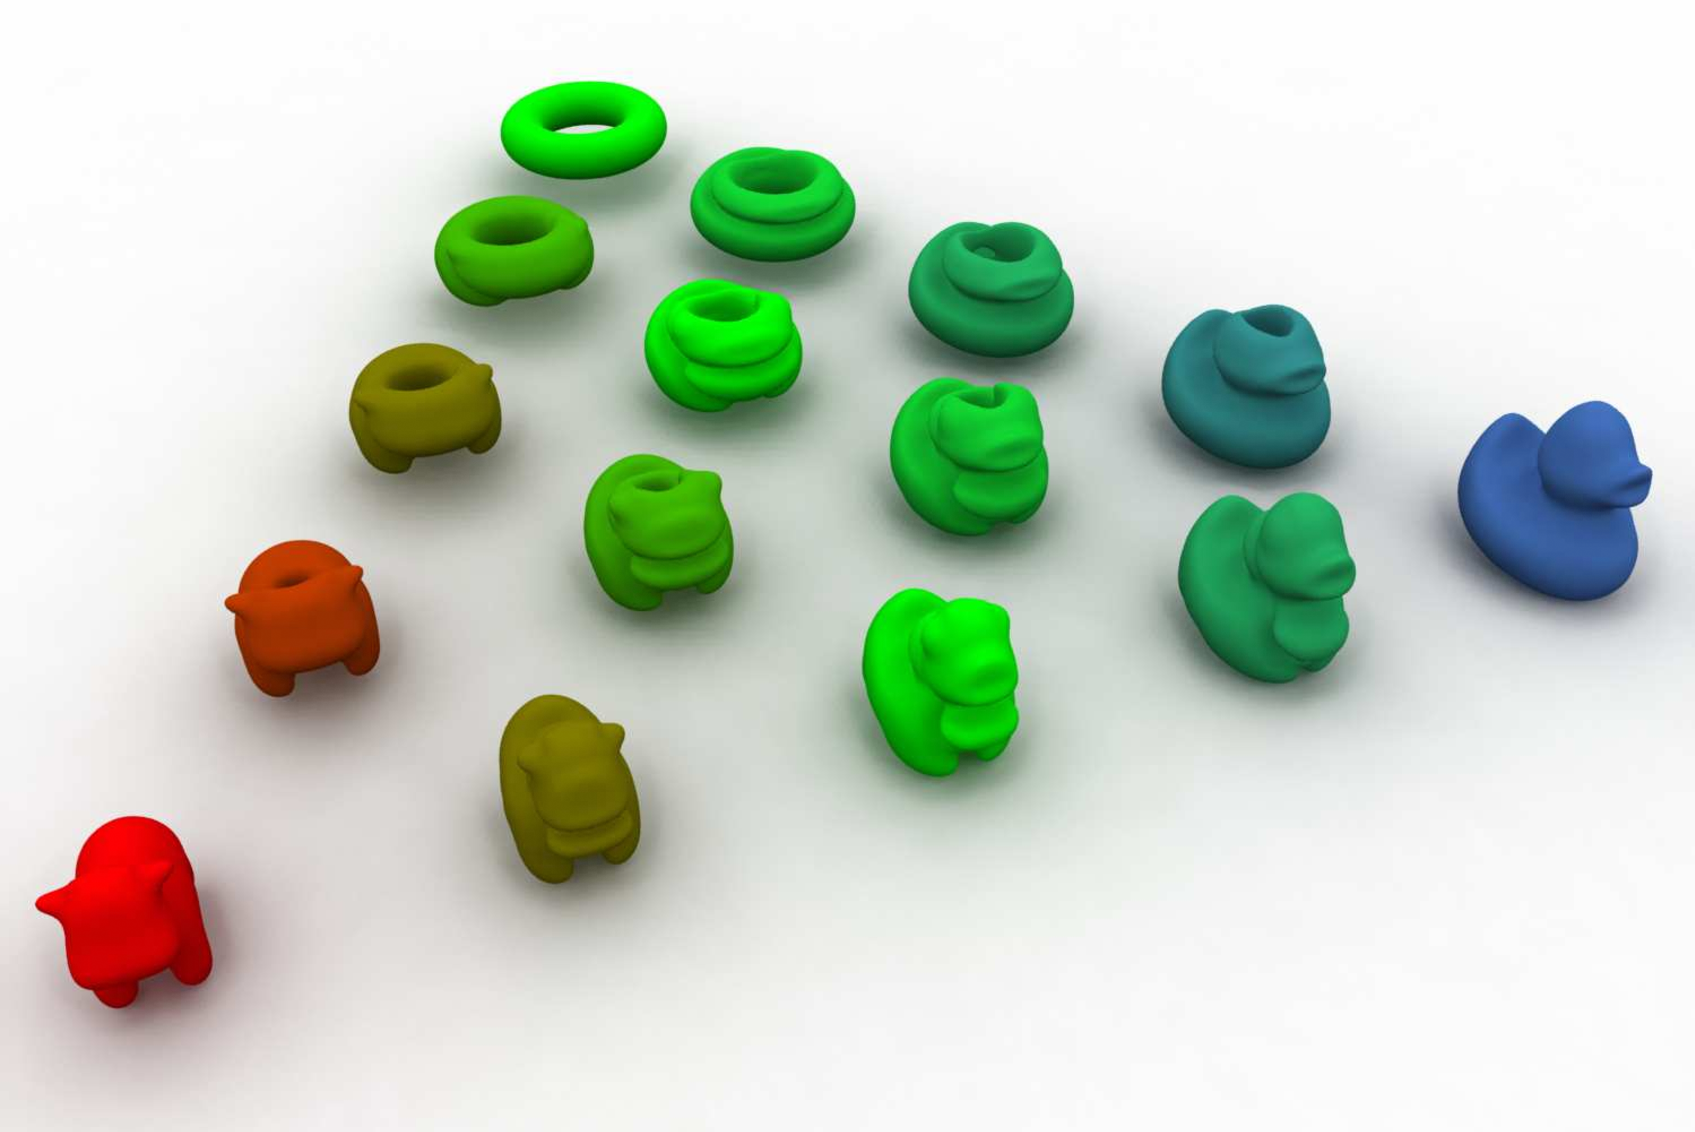
\includegraphics[width=.61\linewidth]{transport-hd/applis/shapes-3d}
\caption{Interpolation barycentrique numérique de formes tridimensionnelles représentées par des distributions de probabilité. Les trois formes de référence occupent les sommets du triangle ; les points intérieurs correspondent à différents poids dans~\eqref{eq-bary}.}\label{fig:barycenters}
\end{figure}

\subsection{Comparer des textes}
Normaliser les nombres d'occurrences des mots d'un texte donne une distribution de probabilité. Le transport compare deux telles distributions à l'aide d'un coût décrivant la dissimilarité entre mots, par exemple une distance entre leurs plongements vectoriels. Le choix de ce coût détermine quelles substitutions sont peu coûteuses ; on peut aussi l'apprendre pour une tâche donnée~\cite{huang2016supervised}. Les histogrammes de mots oublient leur ordre et ne peuvent donc pas, à eux seuls, saisir toutes les distinctions grammaticales ou sémantiques.

\begin{figure}[htbp]\centering

\includegraphics[width=.40\linewidth]{transport-hd/applis/bag-word-1}\hspace{8mm}
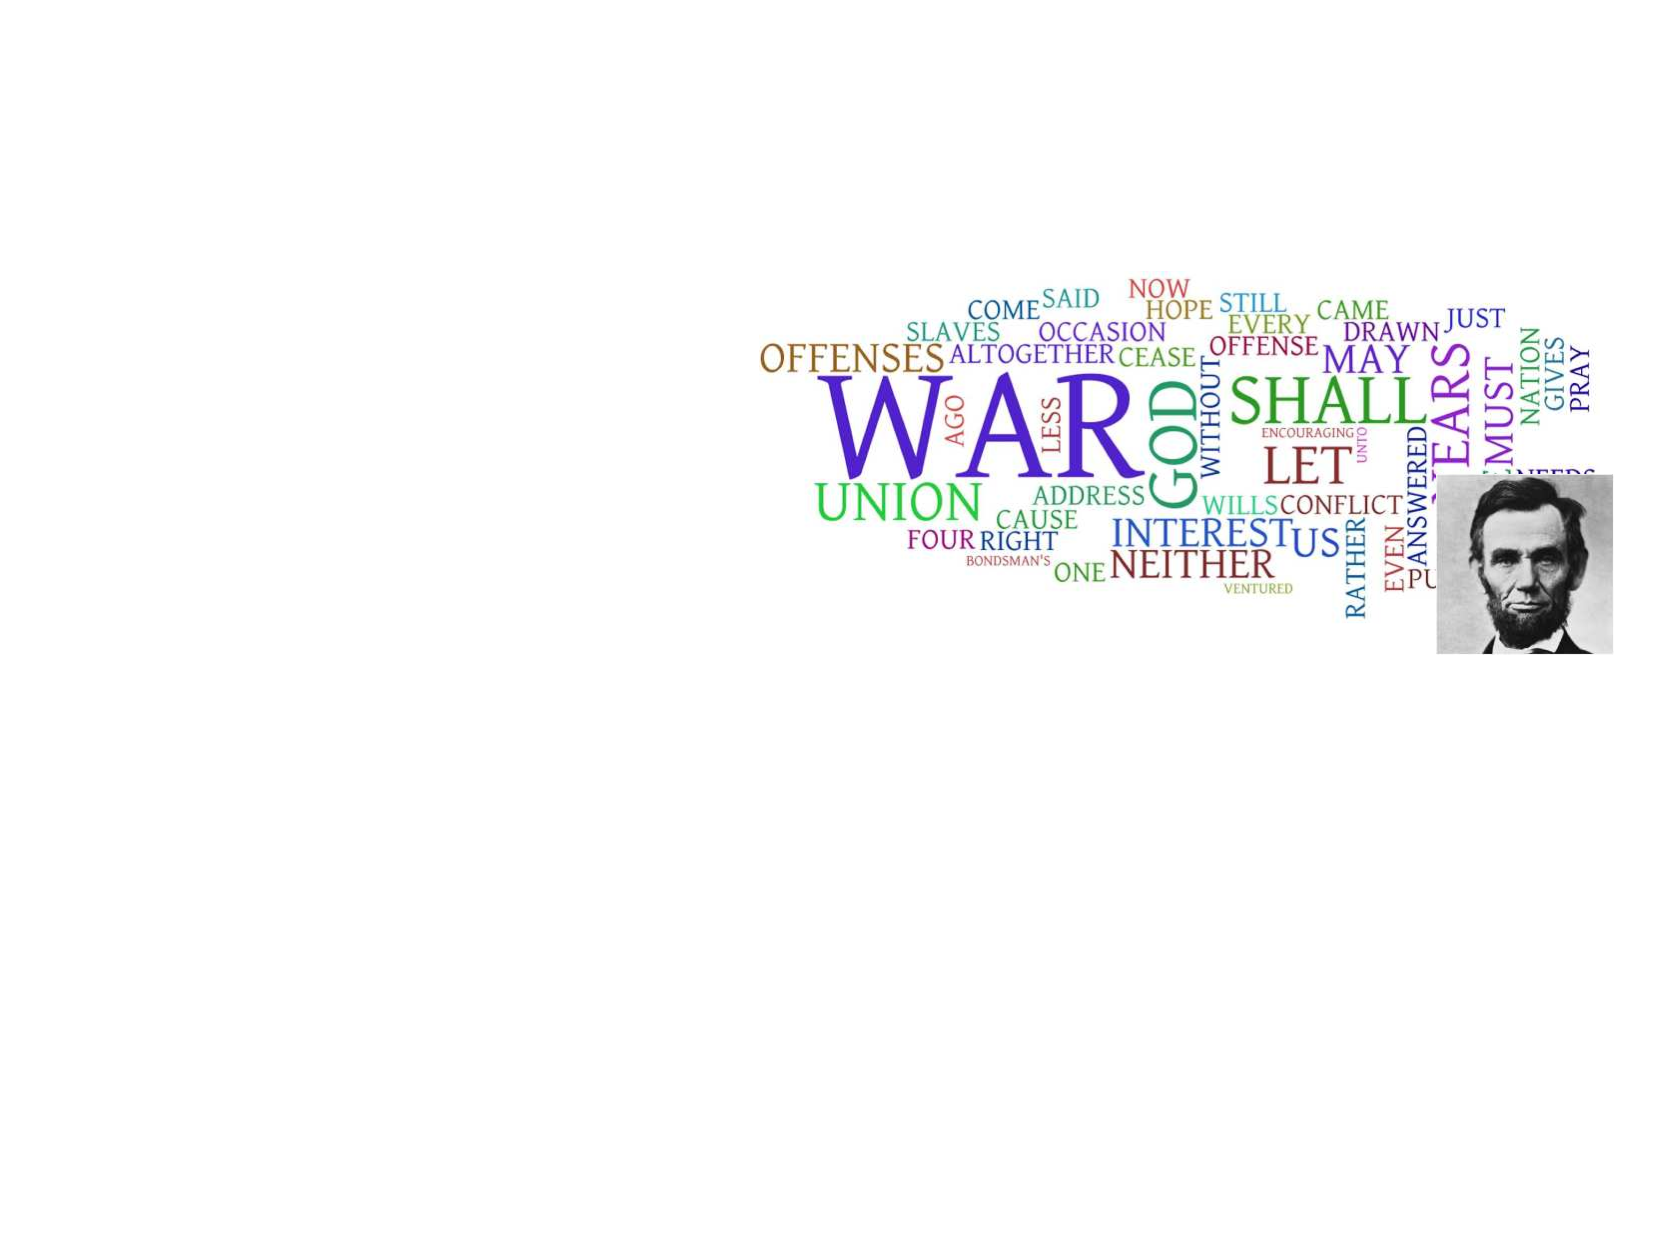
\includegraphics[width=.40\linewidth]{transport-hd/applis/bag-word-2}
\caption{Nuages des mots les plus fréquents de deux textes. Leur taille indique leur fréquence relative ; ces illustrations ne constituent pas un histogramme numérique complet.}\label{fig:bagwords}
\end{figure}

\paragraph*{Pour aller plus loin.}
Pour la théorie, on pourra consulter~\cite{Villani03,SantambrogioBook}. Les méthodes numériques et les applications sont développées dans~\cite{PeyreCuturi}. Le cours \href{https://www.gpeyre.com/ot4ml/}{Optimal Transport for Machine Learning (OT4ML)} propose une autre introduction à ces idées.

\ifdefined\StandaloneChapter
\paragraph*{Remerciements.}
Je remercie Vincent Beck, Gwenn Guichaoua et Marie-Noëlle Peyré pour leurs relectures attentives.
\fi
